% Options for packages loaded elsewhere
\PassOptionsToPackage{unicode}{hyperref}
\PassOptionsToPackage{hyphens}{url}
\documentclass[
]{article}
\usepackage{xcolor}
\usepackage{amsmath,amssymb}
\setcounter{secnumdepth}{-\maxdimen} % remove section numbering
\usepackage{iftex}
\ifPDFTeX
  \usepackage[T1]{fontenc}
  \usepackage[utf8]{inputenc}
  \usepackage{textcomp} % provide euro and other symbols
\else % if luatex or xetex
  \usepackage{unicode-math} % this also loads fontspec
  \defaultfontfeatures{Scale=MatchLowercase}
  \defaultfontfeatures[\rmfamily]{Ligatures=TeX,Scale=1}
\fi
\usepackage{lmodern}
\ifPDFTeX\else
  % xetex/luatex font selection
\fi
% Use upquote if available, for straight quotes in verbatim environments
\IfFileExists{upquote.sty}{\usepackage{upquote}}{}
\IfFileExists{microtype.sty}{% use microtype if available
  \usepackage[]{microtype}
  \UseMicrotypeSet[protrusion]{basicmath} % disable protrusion for tt fonts
}{}
\makeatletter
\@ifundefined{KOMAClassName}{% if non-KOMA class
  \IfFileExists{parskip.sty}{%
    \usepackage{parskip}
  }{% else
    \setlength{\parindent}{0pt}
    \setlength{\parskip}{6pt plus 2pt minus 1pt}}
}{% if KOMA class
  \KOMAoptions{parskip=half}}
\makeatother
\usepackage{graphicx}
\makeatletter
\newsavebox\pandoc@box
\newcommand*\pandocbounded[1]{% scales image to fit in text height/width
  \sbox\pandoc@box{#1}%
  \Gscale@div\@tempa{\textheight}{\dimexpr\ht\pandoc@box+\dp\pandoc@box\relax}%
  \Gscale@div\@tempb{\linewidth}{\wd\pandoc@box}%
  \ifdim\@tempb\p@<\@tempa\p@\let\@tempa\@tempb\fi% select the smaller of both
  \ifdim\@tempa\p@<\p@\scalebox{\@tempa}{\usebox\pandoc@box}%
  \else\usebox{\pandoc@box}%
  \fi%
}
% Set default figure placement to htbp
\def\fps@figure{htbp}
\makeatother
% definitions for citeproc citations
\NewDocumentCommand\citeproctext{}{}
\NewDocumentCommand\citeproc{mm}{%
  \begingroup\def\citeproctext{#2}\cite{#1}\endgroup}
\makeatletter
 % allow citations to break across lines
 \let\@cite@ofmt\@firstofone
 % avoid brackets around text for \cite:
 \def\@biblabel#1{}
 \def\@cite#1#2{{#1\if@tempswa , #2\fi}}
\makeatother
\newlength{\cslhangindent}
\setlength{\cslhangindent}{1.5em}
\newlength{\csllabelwidth}
\setlength{\csllabelwidth}{3em}
\newenvironment{CSLReferences}[2] % #1 hanging-indent, #2 entry-spacing
 {\begin{list}{}{%
  \setlength{\itemindent}{0pt}
  \setlength{\leftmargin}{0pt}
  \setlength{\parsep}{0pt}
  % turn on hanging indent if param 1 is 1
  \ifodd #1
   \setlength{\leftmargin}{\cslhangindent}
   \setlength{\itemindent}{-1\cslhangindent}
  \fi
  % set entry spacing
  \setlength{\itemsep}{#2\baselineskip}}}
 {\end{list}}
\usepackage{calc}
\newcommand{\CSLBlock}[1]{\hfill\break\parbox[t]{\linewidth}{\strut\ignorespaces#1\strut}}
\newcommand{\CSLLeftMargin}[1]{\parbox[t]{\csllabelwidth}{\strut#1\strut}}
\newcommand{\CSLRightInline}[1]{\parbox[t]{\linewidth - \csllabelwidth}{\strut#1\strut}}
\newcommand{\CSLIndent}[1]{\hspace{\cslhangindent}#1}
\setlength{\emergencystretch}{3em} % prevent overfull lines
\providecommand{\tightlist}{%
  \setlength{\itemsep}{0pt}\setlength{\parskip}{0pt}}
\usepackage{bookmark}
\IfFileExists{xurl.sty}{\usepackage{xurl}}{} % add URL line breaks if available
\urlstyle{same}
\hypersetup{
  pdftitle={ESTUDO COMPARATIVO DE ESTRATÉGIAS DE INTEGRAÇÃO PARA AGENTES CONVERSACIONAIS BASEADOS EM IA EM SOLUÇÕES WEB},
  hidelinks,
  pdfcreator={LaTeX via pandoc}}

\title{\textbf{ESTUDO COMPARATIVO DE ESTRATÉGIAS DE INTEGRAÇÃO PARA
AGENTES CONVERSACIONAIS BASEADOS EM IA EM SOLUÇÕES WEB}}
\author{}
\date{}

\begin{document}
\maketitle

\subsubsection{Artigo em produção - Checklist de
produção}\label{artigo-em-produuxe7uxe3o---checklist-de-produuxe7uxe3o}

\begin{itemize}
\tightlist
\item[$\square$]
  Edição do artigo

  \begin{itemize}
  \tightlist
  \item[$\square$]
    Aplicar formatação da SATC

    \begin{itemize}
    \tightlist
    \item[$\square$]
      Definir o template do .docx com o Word
    \end{itemize}
  \item[$\boxtimes$]
    Referências

    \begin{itemize}
    \tightlist
    \item[$\boxtimes$]
      Formatação ABNT
    \end{itemize}
  \end{itemize}
\item[$\square$]
  Escrita

  \begin{itemize}
  \tightlist
  \item[$\boxtimes$]
    Resumo
  \item[$\boxtimes$]
    Introdução
  \item[$\boxtimes$]
    Material e métodos
  \item[$\boxtimes$]
    Revisão e entrega parcial (nota 4.5/5)
  \item[$\square$]
    Desenvolvimento
  \item[$\square$]
    Resultados e discussão
  \item[$\square$]
    Considerações finais
  \item[$\square$]
    Revisão após finalizar o artigo
  \end{itemize}
\end{itemize}

\textbf{Lucas de Castro Zanoni}\footnote{Graduando em Engenharia de
  software no semestre letivo de 2025-1. E-mail:
  castro.lucas290@gmail.com}

\textbf{Thyerri Fernandes Mezzari}\footnote{Professor do Centro
  Universitário UniSATC E-mail: thyerri.mezzari@satc.edu.br}

Resumo: Este trabalho apresenta um estudo experimental comparativo de
abordagens para integração de agentes conversacionais baseados em
inteligência artificial a soluções web. Foram investigadas três
estratégias principais --- integração via plugin ORM, via especificação
OpenAPI com o protocolo Model Context Protocol (MCP) e conexão direta
com banco de dados --- avaliando aspectos como desempenho, segurança,
facilidade de implementação e experiência do usuário. Para garantir uma
análise justa e reprodutível, foi desenvolvida uma interface padronizada
e definidos critérios objetivos, fundamentando-se em referências
acadêmicas, guias de segurança, relatórios de mercado e documentações
oficiais de provedores de modelos de linguagem. O estudo envolveu a
implementação de provas de conceito para cada abordagem, além da
aplicação de testes automatizados end-to-end, com ênfase em métricas de
robustez, segurança (incluindo red teaming e injeção de prompts) e
usabilidade. Os resultados discutem os desafios, vantagens e limitações
de cada alternativa, fornecendo uma análise fundamentada que orienta a
escolha da solução mais adequada conforme o contexto de aplicação.
Assim, este trabalho contribui para o avanço da integração segura e
eficiente de agentes conversacionais em sistemas complexos, promovendo
acessibilidade, usabilidade e confiabilidade.

\textbf{Palavras-chave:} agente conversacional, integração de sistemas,
inteligência artificial, segurança, usabilidade.

\section{1 INTRODUÇÃO}\label{introduuxe7uxe3o}

A evolução das interfaces de usuário tem gerado uma diversidade de
padrões de design e usabilidade, resultando frequentemente em barreiras
para a plena acessibilidade e interação dos usuários com os sistemas
digitais. Com o aumento da complexidade do frontend e a multiplicidade
de paradigmas de interação, muitos usuários enfrentam dificuldades
significativas para utilizar efetivamente as funcionalidades oferecidas
pelas soluções web modernas (RAPP et al., 2018) (KOCABALLI et al.,
2019). Nesse contexto, a ascensão dos Modelos de Linguagem de Grande
Escala (LLMs), como os desenvolvidos por OpenAI, Anthropic e Google, tem
impulsionado o desenvolvimento de agentes conversacionais mais avançados
e adaptáveis (ANTHROPIC, 2024a; OPENAI, 2022). Nos últimos anos, avanços
em modelos baseados em Transformer, como o BERT (2018), que aprimorou a
compreensão textual, e o GPT-3 (2020), que ampliou as capacidades
generativas e o aprendizado com poucos exemplos (\emph{few-shot}),
permitiram que os LLMs realizassem tarefas cada vez mais complexas a
partir de simples instruções em linguagem natural. Esses avanços
consolidaram os LLMs como interfaces conversacionais robustas e eficazes
para integração com sistemas.

Diante desse cenário, estudos recentes têm demonstrado que agentes
conversacionais podem aprimorar significativamente a experiência do
usuário ao simplificar interações com sistemas complexos (FAST et al.,
2017). Além disso, a implementação de interfaces baseadas em linguagem
natural tem mostrado potencial para melhorar a usabilidade em contextos
domésticos e inteligentes, reduzindo o tempo e o esforço necessários
para completar tarefas complexas (GUO et al., 2024). Ademais, tais
interfaces oferecem vantagens consideráveis em termos de acessibilidade,
permitindo uma comunicação mais inclusiva e adaptável a usuários com
diferentes necessidades especiais (LISTER et al., 2020) (DENG, 2023).
Para que esses benefícios sejam efetivamente alcançados em soluções web,
é fundamental avaliar as diferentes estratégias de integração desses
agentes aos sistemas existentes.

Nesse sentido, este estudo aborda experimentalmente três estratégias
distintas para integrar agentes conversacionais baseados em IA a
sistemas web: integração via plugins ORM, que utilizam camadas de
abstração para acesso simplificado aos dados; integração por meio de
APIs seguindo a especificação OpenAPI com o protocolo emergente MCP
(Model Context Protocol), focado em interfaces padronizadas; e conexão
direta com banco de dados, permitindo interações sem intermediários
adicionais. Essas abordagens serão avaliadas comparativamente,
destacando suas particularidades quanto a desempenho, segurança,
facilidade de implementação e experiência do usuário.

Dessa forma, a problemática central desta pesquisa reside na questão: de
que forma um agente conversacional baseado em IA pode potencializar a
interação entre usuários e sistemas, promovendo uma comunicação fluida
mesmo em ambientes com interfaces complexas? Essa pergunta reflete a
necessidade crescente de soluções que democratizem o acesso à
tecnologia, reduzindo a curva de aprendizado necessária para a
utilização de sistemas especializados e tornando-os mais acessíveis para
diferentes perfis de usuários.

A relevância deste estudo evidencia-se pelo potencial transformador que
os agentes conversacionais representam para a área de interação
humano-computador. Ao implementar um sistema intermediário capaz de
interpretar linguagem natural e traduzi-la em ações específicas dentro
de um sistema, cria-se uma ponte que permite aos usuários interagir de
forma mais intuitiva e natural com as tecnologias digitais. Esta
abordagem tem o potencial de mitigar as barreiras impostas por
interfaces complexas, contribuindo para uma maior inclusão digital e
para a melhoria da experiência do usuário em diversos contextos de
aplicação.

\section{2 PROCEDIMENTO EXPERIMENTAL}\label{procedimento-experimental}

Este estudo adota uma abordagem experimental estruturada em etapas
sequenciais para investigar comparativamente as três estratégias de
integração mencionadas anteriormente: integração via plugins ORM,
integração por meio de APIs seguindo a especificação OpenAPI com o
protocolo MCP, e conexão direta com banco de dados. Cada abordagem será
examinada com base em provas de conceito práticas, desenvolvidas para
validar sua viabilidade técnica e avaliar objetivamente aspectos
funcionais e não-funcionais.

Inicialmente, será conduzida uma revisão sistemática da literatura,
consolidando conhecimentos científicos sobre cada abordagem e embasando
teoricamente a fase experimental. Na sequência, cada estratégia será
implementada e testada por meio de provas de conceito específicas,
garantindo a padronização das interfaces e condições de avaliação.

Os critérios de avaliação definidos incluem desempenho, segurança,
facilidade de implementação, manutenibilidade e experiência do usuário.
Para assegurar resultados objetivos e comparáveis, os testes incluirão
análises automatizadas end-to-end, medidas de robustez e segurança (como
testes de red teaming e proteção contra injeção de prompts) e avaliações
qualitativas de usabilidade. Os resultados serão sistematicamente
documentados e analisados, permitindo identificar desafios, vantagens e
limitações intrínsecas a cada método de integração e facilitando a
tomada de decisão quanto à abordagem mais adequada para diferentes
contextos de aplicação.

\subsection{2.1 MATERIAIS}\label{materiais}

Para garantir a rigorosidade científica e a reprodutibilidade dos
experimentos conduzidos neste estudo, é essencial uma seleção criteriosa
dos materiais e ferramentas utilizados. Esta seção detalha os recursos
específicos empregados na condução desta pesquisa, justificando sua
escolha baseada na eficiência, popularidade, robustez e aplicabilidade
prática dentro do contexto dos agentes conversacionais e integração de
sistemas.

\subsubsection{2.1.1 NODE.JS PARA DESENVOLVIMENTO DAS PROVAS DE
CONCEITO}\label{node.js-para-desenvolvimento-das-provas-de-conceito}

Node.js foi escolhido como plataforma principal para o desenvolvimento
das provas de conceito devido à sua comprovada eficácia na integração de
sistemas baseados em inteligência artificial (IA), especialmente com
agentes conversacionais e LLMs. A plataforma é amplamente adotada devido
à sua arquitetura orientada a eventos e capacidade de gerenciar
eficientemente múltiplas conexões simultâneas, essencial para aplicações
que exigem respostas rápidas em tempo real (CHEREDNICHENKO et al.,
2024).

Relatórios da \emph{Red Hat} destacam que o uso eficiente da arquitetura
assíncrona do Node.js possibilita a criação de agentes baseados em LLMs
com alta performance e escalabilidade. Isso garante um gerenciamento
eficiente de múltiplas operações paralelas, essencial para aplicações
intensivas em IA e integração com APIs externas (BLOG, 2024).

\subsubsection{\texorpdfstring{2.1.2 TESTES \emph{END-TO-END}
(E2E)}{2.1.2 TESTES END-TO-END (E2E)}}\label{testes-end-to-end-e2e}

O \emph{Framework} de Gerenciamento de Riscos de IA do NIST (OPREA;
VASSILEV, 2023) destaca a importância de avaliar o desempenho de
sistemas de IA de forma abrangente, defendendo que testes de integração
devem avaliar os sistemas de ponta a ponta para identificar erros de
integração e garantir a precisão das respostas em cenários realistas.
Testes rigorosos como esses não apenas identificam problemas de
integração, mas também asseguram às partes interessadas que o sistema se
comporta conforme o esperado em condições do mundo real.

A injeção de \emph{prompt} representa um risco significativo em
implantações de LLMs em nosso cenário, no qual o modelo possui acesso a
dados e sistemas potencialmente críticos, incluindo, ocasionalmente,
conexões diretas com dados brutos de banco de dados. O guia de riscos da
OWASP (JOHN et al., 2025) classifica a injeção de \emph{prompt} como uma
ameaça crítica à segurança, destacando a necessidade de procedimentos de
teste rigorosos para garantir que agentes conversacionais baseados em
LLMs não revelem inadvertidamente dados sensíveis ou contornem
restrições do sistema quando expostos a entradas maliciosas.
Recentemente, Wu et al.~(2023) (WU et al., 2023) demonstraram que
ataques de \emph{jailbreak} --- um tipo avançado de injeção de
\emph{prompt} --- podem burlar as salvaguardas éticas de modelos como o
ChatGPT em até 67\% dos casos, gerando conteúdos prejudiciais como
extorsão e desinformação.

Com isso em mente, o uso de testes E2E pode ser utilizado para avaliar a
resiliência da implementação ao simular entradas adversárias, processo
conhecido como \emph{red teaming}. Segundo Inie et al.~(2025) (INIE;
STRAY; DERCZYNSKI, 2025), o \emph{red teaming} desafia sistematicamente
sistemas de IA com \emph{prompts} adversários projetados para testar
seus limites e mecanismos de segurança. Ao encapsular consultas do
usuário com lembretes de responsabilidade ética (e.g., ``Você deve ser
um ChatGPT responsável''), o método reduziu a taxa de sucesso de
\emph{jailbreaks} para 19\%, mantendo a funcionalidade padrão do modelo
--- um resultado validado através de testes E2E em 540 cenários
adversarialmente projetados (WU et al., 2023).

\subsubsection{2.1.3 MODELOS DE LINGUAGEM DE GRANDE ESCALA
(LLMs)}\label{modelos-de-linguagem-de-grande-escala-llms}

Os LLMs, incluindo tecnologias como OpenAI GPT, Anthropic e modelos
disponibilizados pela Google, são essenciais neste estudo devido à sua
capacidade de interpretar e gerar linguagem natural de forma avançada e
eficaz. Estes modelos foram selecionados por sua performance comprovada
e ampla adoção em pesquisas acadêmicas e no mercado corporativo,
proporcionando um sólido embasamento para as funcionalidades de
interação do agente conversacional.

\paragraph{2.1.3.1 HISTÓRICO DO DESENVOLVIMENTO DE LLMS
(2018--2023)}\label{histuxf3rico-do-desenvolvimento-de-llms-20182023}

Nos últimos cinco anos, os LLMs evoluíram rapidamente, a partir da
arquitetura Transformer. O lançamento do BERT (2018) mostrou avanços em
compreensão textual, enquanto a série GPT demonstrou fortes capacidades
generativas. O GPT-3 (2020), com 175 bilhões de parâmetros, evidenciou
habilidades emergentes de aprendizado com poucos exemplos
(\emph{few-shot}), ampliando o escopo de tarefas possíveis por meio de
simples instruções em linguagem natural (BROWN et al., 2020).

A partir de 2022, o foco da pesquisa passou a ser o aprimoramento do
raciocínio e alinhamento dos LLMs. Técnicas como \emph{Chain-of-Thought
prompting} permitiram que os modelos resolvessem problemas complexos de
forma mais eficaz (WEI et al., 2023). O uso de Reinforcement Learning
from Human Feedback (RLHF), como nos modelos InstructGPT e
posteriormente ChatGPT, melhorou a capacidade dos LLMs de seguir
instruções com mais segurança e consistência. Esses avanços
estabeleceram as bases para o uso dos LLMs como interfaces
conversacionais robustas em cenários de integração com sistemas (OPENAI,
2022).

\paragraph{2.1.3.2 EXTENSÃO DE JANELA DE
CONTEXTO}\label{extensuxe3o-de-janela-de-contexto}

Com o avanço dos modelos, observou-se uma tendência significativa no
aumento das janelas de contexto --- a quantidade de tokens que um LLM
pode processar em uma única interação. Modelos como o Claude 3 já
alcançam até 100.000 tokens (ANTHROPIC, 2024b), enquanto versões
estendidas do GPT-4 suportam até 32.000 tokens (OPENAI, 2023a). Esse
aumento permite que os modelos processem documentos extensos, múltiplas
conversas ou grandes volumes de dados em uma única solicitação,
superando, em muitos casos, abordagens tradicionais baseadas em
retrieval-augmented generation (RAG), especialmente em tarefas que
exigem síntese contextual profunda.

A capacidade de manter longos contextos é altamente benéfica para
integração com sistemas -- um LLM pode manter diálogos prolongados,
lembrar estados extensos ou ingerir bancos de dados e logs inteiros de
uma só vez. No entanto, isso traz custos computacionais consideráveis, e
há esforços contínuos para utilizar essas janelas maiores de forma
eficiente (por exemplo, condensando ou focando a atenção nas partes mais
relevantes) (ANTHROPIC, 2024b; OPENAI, 2023a).

\paragraph{2.1.3.3 RACIOCÍNIO APRIMORADO E COMPREENSÃO PROFUNDA (DEEP
THINKING)}\label{raciocuxednio-aprimorado-e-compreensuxe3o-profunda-deep-thinking}

Os LLMs mais recentes apresentam avanços significativos em raciocínio,
planejamento e resolução de tarefas complexas. Técnicas como o
\emph{Chain-of-Thought prompting}, que induz os modelos a pensar em
etapas intermediárias, mostraram ganhos substanciais em tarefas que
exigem múltiplos passos lógicos (WEI et al., 2023). Além disso,
abordagens como \emph{tree-of-thought} e \emph{self-reflection} permitem
que os modelos reavaliem suas respostas e melhorem sua própria
performance iterativamente. Esses avanços tornam os LLMs mais confiáveis
para tarefas que exigem raciocínio profundo e tomada de decisão
estruturada, fundamentais para integração com sistemas complexos (YAO et
al., 2023).

\paragraph{2.1.3.4 USO DE FERRAMENTAS EM TEMPO REAL E INTERAÇÃO COM
SISTEMAS}\label{uso-de-ferramentas-em-tempo-real-e-interauxe7uxe3o-com-sistemas}

O avanço dos LLMs em ambientes de produção foi impulsionado por recursos
como o \emph{function calling} da OpenAI. Essa funcionalidade permite
que os modelos interpretem solicitações em linguagem natural e as
convertam em chamadas de funções estruturadas, conforme definido pelo
desenvolvedor. Por exemplo, ao receber uma instrução como ``agende uma
reunião para amanhã às 14h'', o modelo pode gerar uma chamada de função
com os parâmetros apropriados para interagir com uma API de calendário,
sem depender de engenharia de \emph{prompt} ou extração de texto
(OPENAI, 2023b). Essa abordagem, melhora significativamente a
confiabilidade em cenários de integração, permitindo que o modelo
obtenha dados estruturados de bancos de dados, chame APIs de negócios,
envie e-mails, entre outras ações, em vez de apenas tentar adivinhar a
resposta (OPENAI, 2023b).

Complementando essa capacidade, o \emph{Model Context Protocol} (MCP),
desenvolvido pela Anthropic (ANTHROPIC, 2024a; MODEL CONTEXT PROTOCOL
TEAM, 2025), oferece um padrão aberto para conectar LLMs a diversas
fontes de dados e ferramentas. O MCP estabelece uma arquitetura
cliente-servidor onde os modelos (clientes) podem acessar servidores MCP
que expõem recursos, \emph{prompts} e ferramentas de forma padronizada.
Isso elimina a necessidade de integrações personalizadas para cada fonte
de dados, promovendo uma interoperabilidade mais ampla e sustentável.

\subsubsection{2.1.4 FERRAMENTAS ESPECÍFICAS DE
INTEGRAÇÃO}\label{ferramentas-especuxedficas-de-integrauxe7uxe3o}

A pesquisa investigou quatro abordagens distintas para a integração dos
agentes conversacionais com soluções \emph{web}, utilizando ferramentas
específicas para cada uma:

\begin{itemize}
\item
  \textbf{PostgreSQL para Conexão Direta com Banco de Dados:} foi
  escolhido para a conexão direta com banco de dados devido à sua ampla
  adoção e aceitação pela comunidade de desenvolvedores, evidenciada
  pela pesquisa do \emph{Stack Overflow Developer Survey}, onde apareceu
  como o banco de dados mais admirado e desejado por desenvolvedores em
  2023 (ENTERPRISEDB, 2023a). Além disso, décadas de desenvolvimento
  ativo e testes rigorosos pela comunidade garantem ao PostgreSQL uma
  reputação sólida em termos de integridade dos dados e tolerância a
  falhas. Assim, utilizar PostgreSQL assegura que os dados do agente
  conversacional sejam gerenciados por uma infraestrutura confiável,
  escalável e amplamente reconhecida pela indústria, com vasto suporte
  operacional disponível (ENTERPRISEDB, 2023a, 2023b).
\item
  \textbf{Sequelize para Integração via ORM:} Este ORM foi selecionado
  como ferramenta ORM devido ao seu amplo uso em aplicações Node.js,
  sendo uma das bibliotecas mais populares para gerenciamento de banco
  de dados nessa plataforma, com cerca de 27 mil estrelas no GitHub e
  mais de meio milhão de repositórios que o utilizam (TEAM, 2024).
  Empresas reconhecidas, como PayPal e Red Hat, utilizam Sequelize em
  produção, reforçando sua credibilidade e robustez. Além disso, o uso
  de Sequelize proporciona segurança adicional ao prevenir
  automaticamente ataques de \emph{SQL injection} por meio de queries
  parametrizadas, oferecendo também suporte para caches e consultas em
  SQL bruto quando necessário, equilibrando segurança com flexibilidade
  e desempenho (TEAM, 2023).
\item
  \textbf{OpenAPI para Integração com Swagger:} foi selecionado devido à
  sua ampla adoção como padrão da indústria para definição de interfaces
  \emph{RESTful}, sendo reconhecido por facilitar a documentação
  consistente e interoperabilidade entre sistemas. Sua especificação
  permite descrever de maneira clara e estruturada os contratos das
  APIs, incluindo esquemas de autenticação como OAuth e chaves de API,
  essenciais para declarar uniformemente os requisitos de segurança das
  interfaces dos agentes conversacionais (OPENAPI INITIATIVE, 2023; THE
  POSTMAN TEAM, 2023).
\end{itemize}

A relevância do OpenAPI para agentes baseados em LLM reside na
possibilidade de fornecer uma descrição estruturada das capacidades
disponíveis para o agente. Por meio de uma definição formal e
padronizada, os modelos de linguagem podem interpretar diretamente as
interfaces, compreendendo quais operações podem ser solicitadas e como
realizá-las com segurança e eficiência. Essa abordagem já é aplicada por
sistemas como os plugins do ChatGPT, demonstrando sua efetividade para
integração direta entre LLMs e APIs externas (OPENAI, 2023c).

\begin{itemize}
\tightlist
\item
  \textbf{Model Context Protocol (MCP):} é um padrão aberto emergente
  para integração entre agentes de IA e sistemas externos, com o
  objetivo de padronizar como modelos acessam dados, serviços e
  ferramentas. Ele fornece uma arquitetura clara baseada em clientes e
  servidores, permitindo que agentes conversem com fontes externas de
  forma segura, modular e escalável. Desde seu lançamento aberto, no
  final de novembro de 2024, o protocolo ganhou tração significativa com
  a criação de diversos servidores prontos para PostgreSQL, GitHub,
  Slack, entre outros, além de SDKs em múltiplas linguagens (ANTHROPIC,
  2024c; MODEL CONTEXT PROTOCOL CONTRIBUTORS, 2024).
\end{itemize}

A adoção crescente é impulsionada pela comunidade ativa, o que demonstra
o potencial do MCP como um padrão de integração para sistemas baseados
em LLMs. Sua proposta de `porta universal' para conectar agentes a
ferramentas oferece flexibilidade e segurança: características
fundamentais quando agentes com poder de raciocínio, como LLMs, precisam
acessar recursos sensíveis de forma controlada e auditável (ANTHROPIC,
2024c).

\subsection{2.2 MÉTODOS}\label{muxe9todos}

Para assegurar a rigorosidade científica e garantir a reprodutibilidade
dos experimentos conduzidos neste estudo, foi desenvolvida uma interface
padrão comum para avaliar todas as abordagens de integração. Essa
padronização viabiliza uma comparação justa e objetiva entre as
implementações, minimizando variáveis relacionadas à interface que
poderiam interferir nos resultados finais.

\subsubsection{2.2.1 Interface Comum de
Usuário}\label{interface-comum-de-usuuxe1rio}

A interface comum consiste em uma aplicação \emph{web} simples de chat,
desenvolvida utilizando React.js e TypeScript. A interface foi projetada
de forma minimalista, visando uma experiência consistente e objetiva,
independentemente da abordagem de integração utilizada.

\begin{figure}
\centering
\pandocbounded{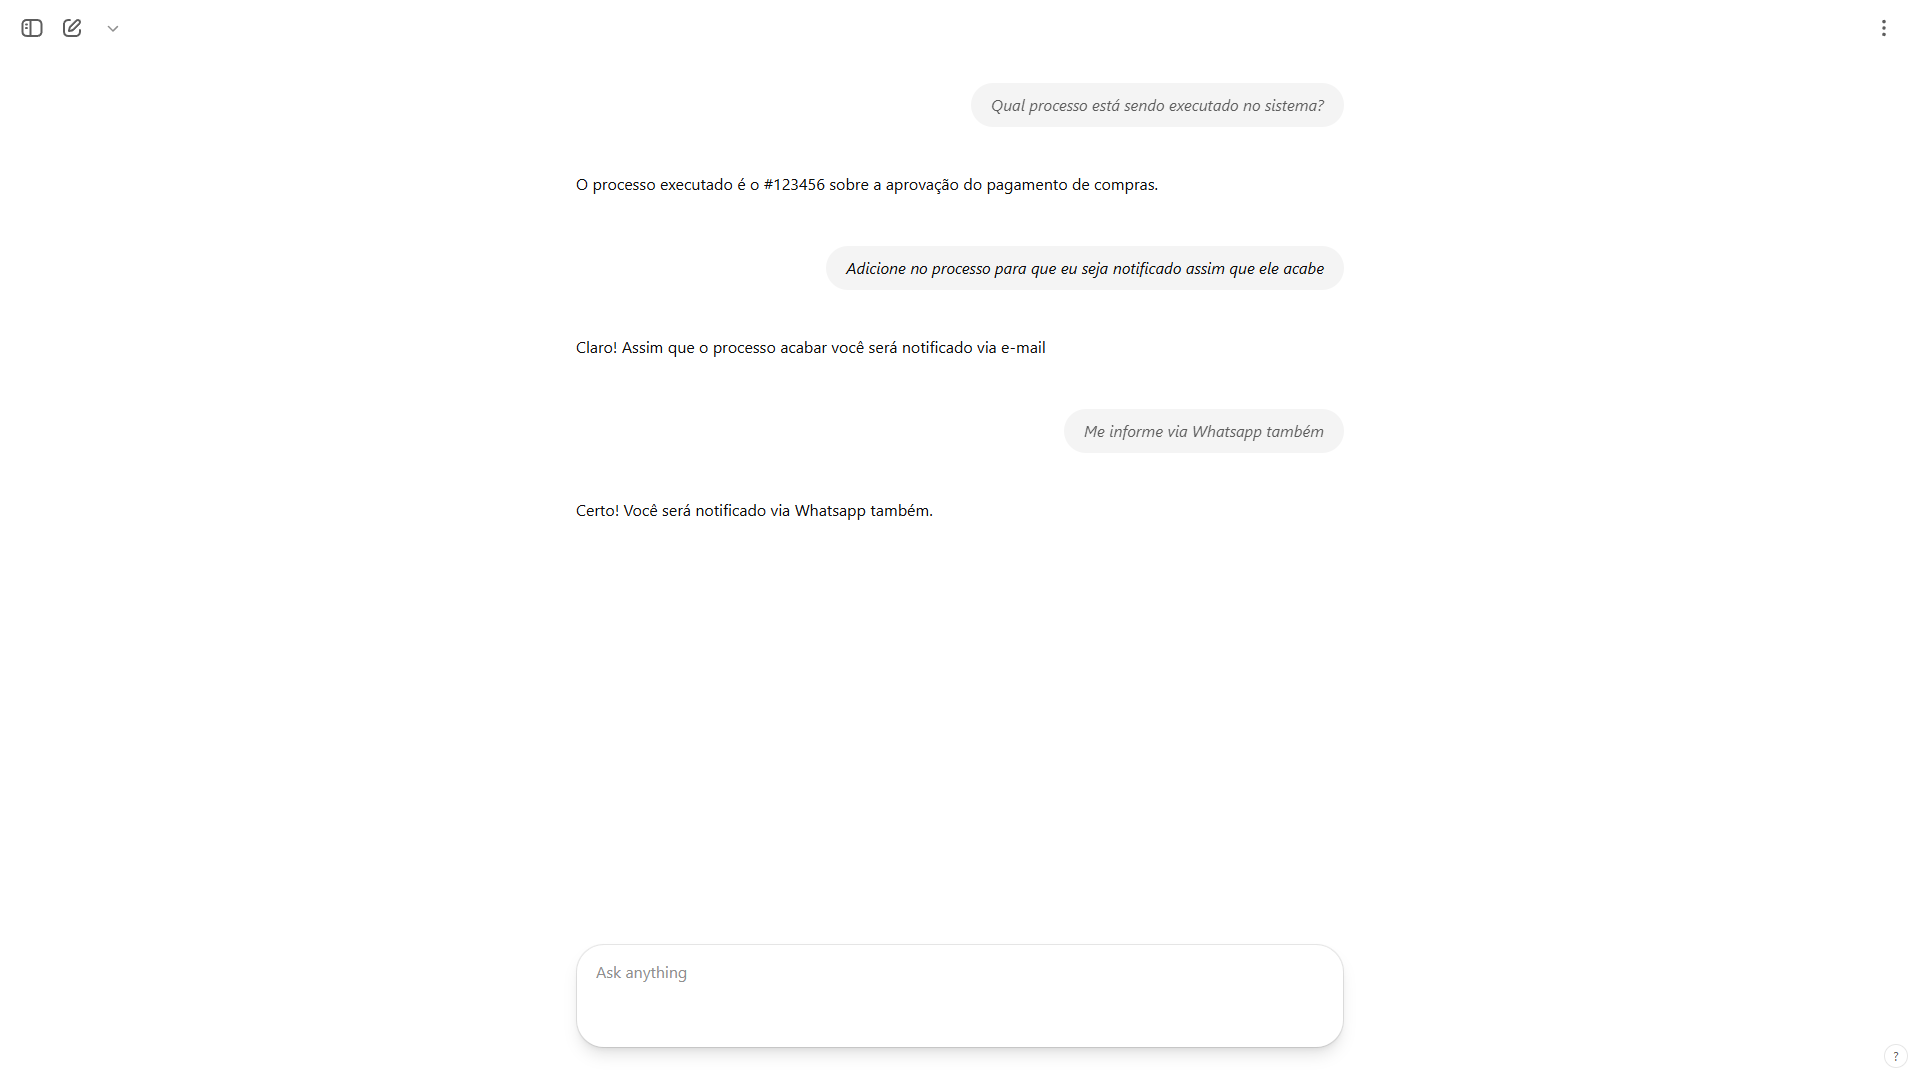
\includegraphics[keepaspectratio]{images/metodos/user-interface.jpg}}
\caption{Interface do Usuário}
\end{figure}

\paragraph{2.2.1.1 DESIGN DA INTERFACE}\label{design-da-interface}

A interface é composta por uma seção principal que exibe o histórico de
mensagens, onde as interações entre usuário e agente conversacional
aparecem de forma intercalada: as mensagens do agente são exibidas à
esquerda e as do usuário à direita, facilitando a distinção visual entre
os participantes da conversa. Abaixo do histórico, há um campo de
entrada de texto que permite ao usuário digitar e enviar novas
mensagens. Esse layout possibilita ao usuário acompanhar facilmente todo
o histórico da conversa e inserir novos \emph{prompts} de maneira
contínua e intuitiva.

\paragraph{2.2.1.2 Comunicação com
Backend}\label{comunicauxe7uxe3o-com-backend}

A comunicação entre frontend e backend será estabelecida por meio de uma
API REST síncrona, simplificando o processo de envio e retorno de
mensagens. Cada consulta feita pelo usuário gerará uma única requisição
ao backend que processará integralmente essa requisição utilizando um
LLM e devolverá uma resposta após concluir o processamento, mantendo o
fluxo de comunicação claro e previsível.

\subsubsection{2.2.2 Arquitetura e Fluxo de Integração do
Sistema}\label{arquitetura-e-fluxo-de-integrauxe7uxe3o-do-sistema}

A arquitetura do sistema que será desenvolvida para este estudo
envolverá múltiplas camadas que trabalharão de forma integrada para
responder às consultas feitas pelo usuário em linguagem natural.
Inicialmente, as consultas serão recebidas pela interface \emph{web} e
encaminhadas ao backend, onde o modelo de linguagem executará o processo
de análise e interpretação.

\begin{figure}
\centering
\pandocbounded{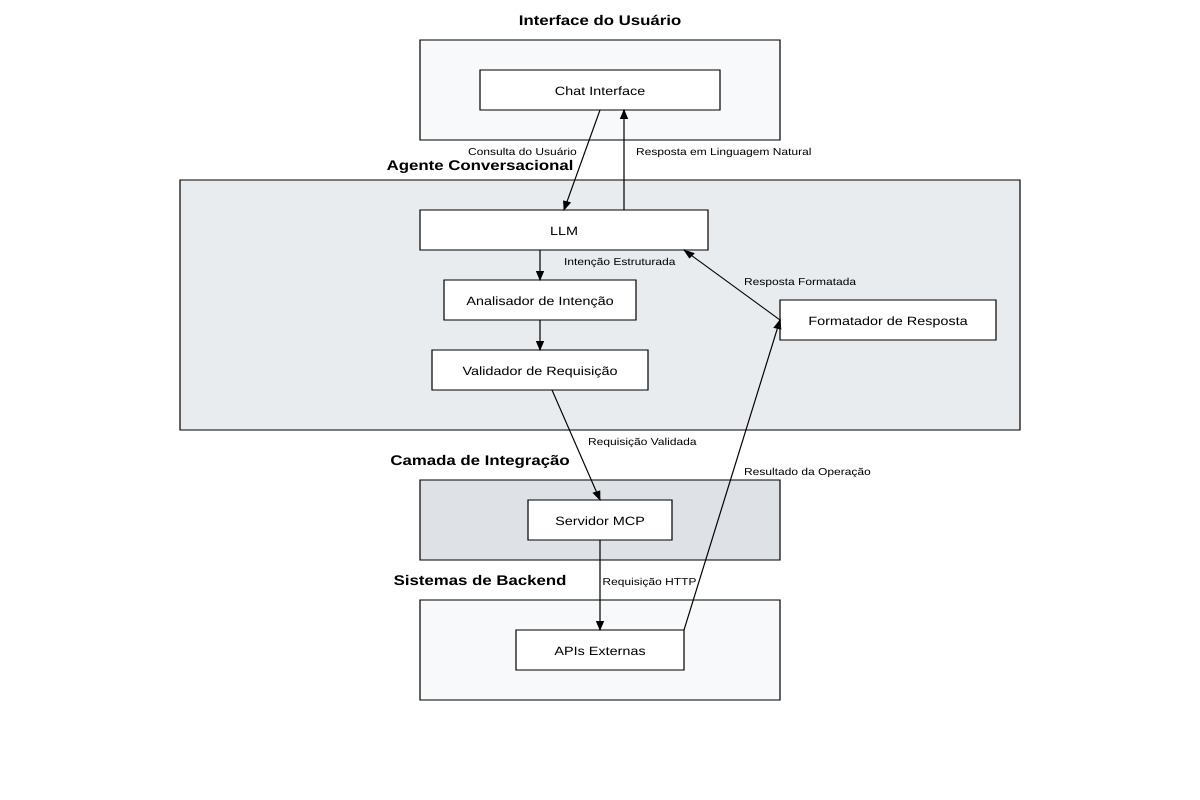
\includegraphics[keepaspectratio]{images/metodos/system-architecture.jpg}}
\caption{Arquitetura do Sistema}
\end{figure}

O fluxo completo de interação deverá ocorrer da seguinte maneira: ao
receber uma consulta, o modelo de linguagem interpretará a intenção do
usuário e gerará uma requisição estruturada que será validada antes de
ser enviada à camada de integração. Essa camada utilizará diferentes
abordagens (ORM, MCP ou conexão direta com o banco de dados) para
acessar sistemas backend, como modelos de dados, APIs externas ou bancos
de dados diretamente. Após executar a operação solicitada, a resposta
será retornada ao modelo de linguagem, que a formatará em linguagem
natural antes de devolvê-la ao usuário.

\begin{figure}
\centering
\pandocbounded{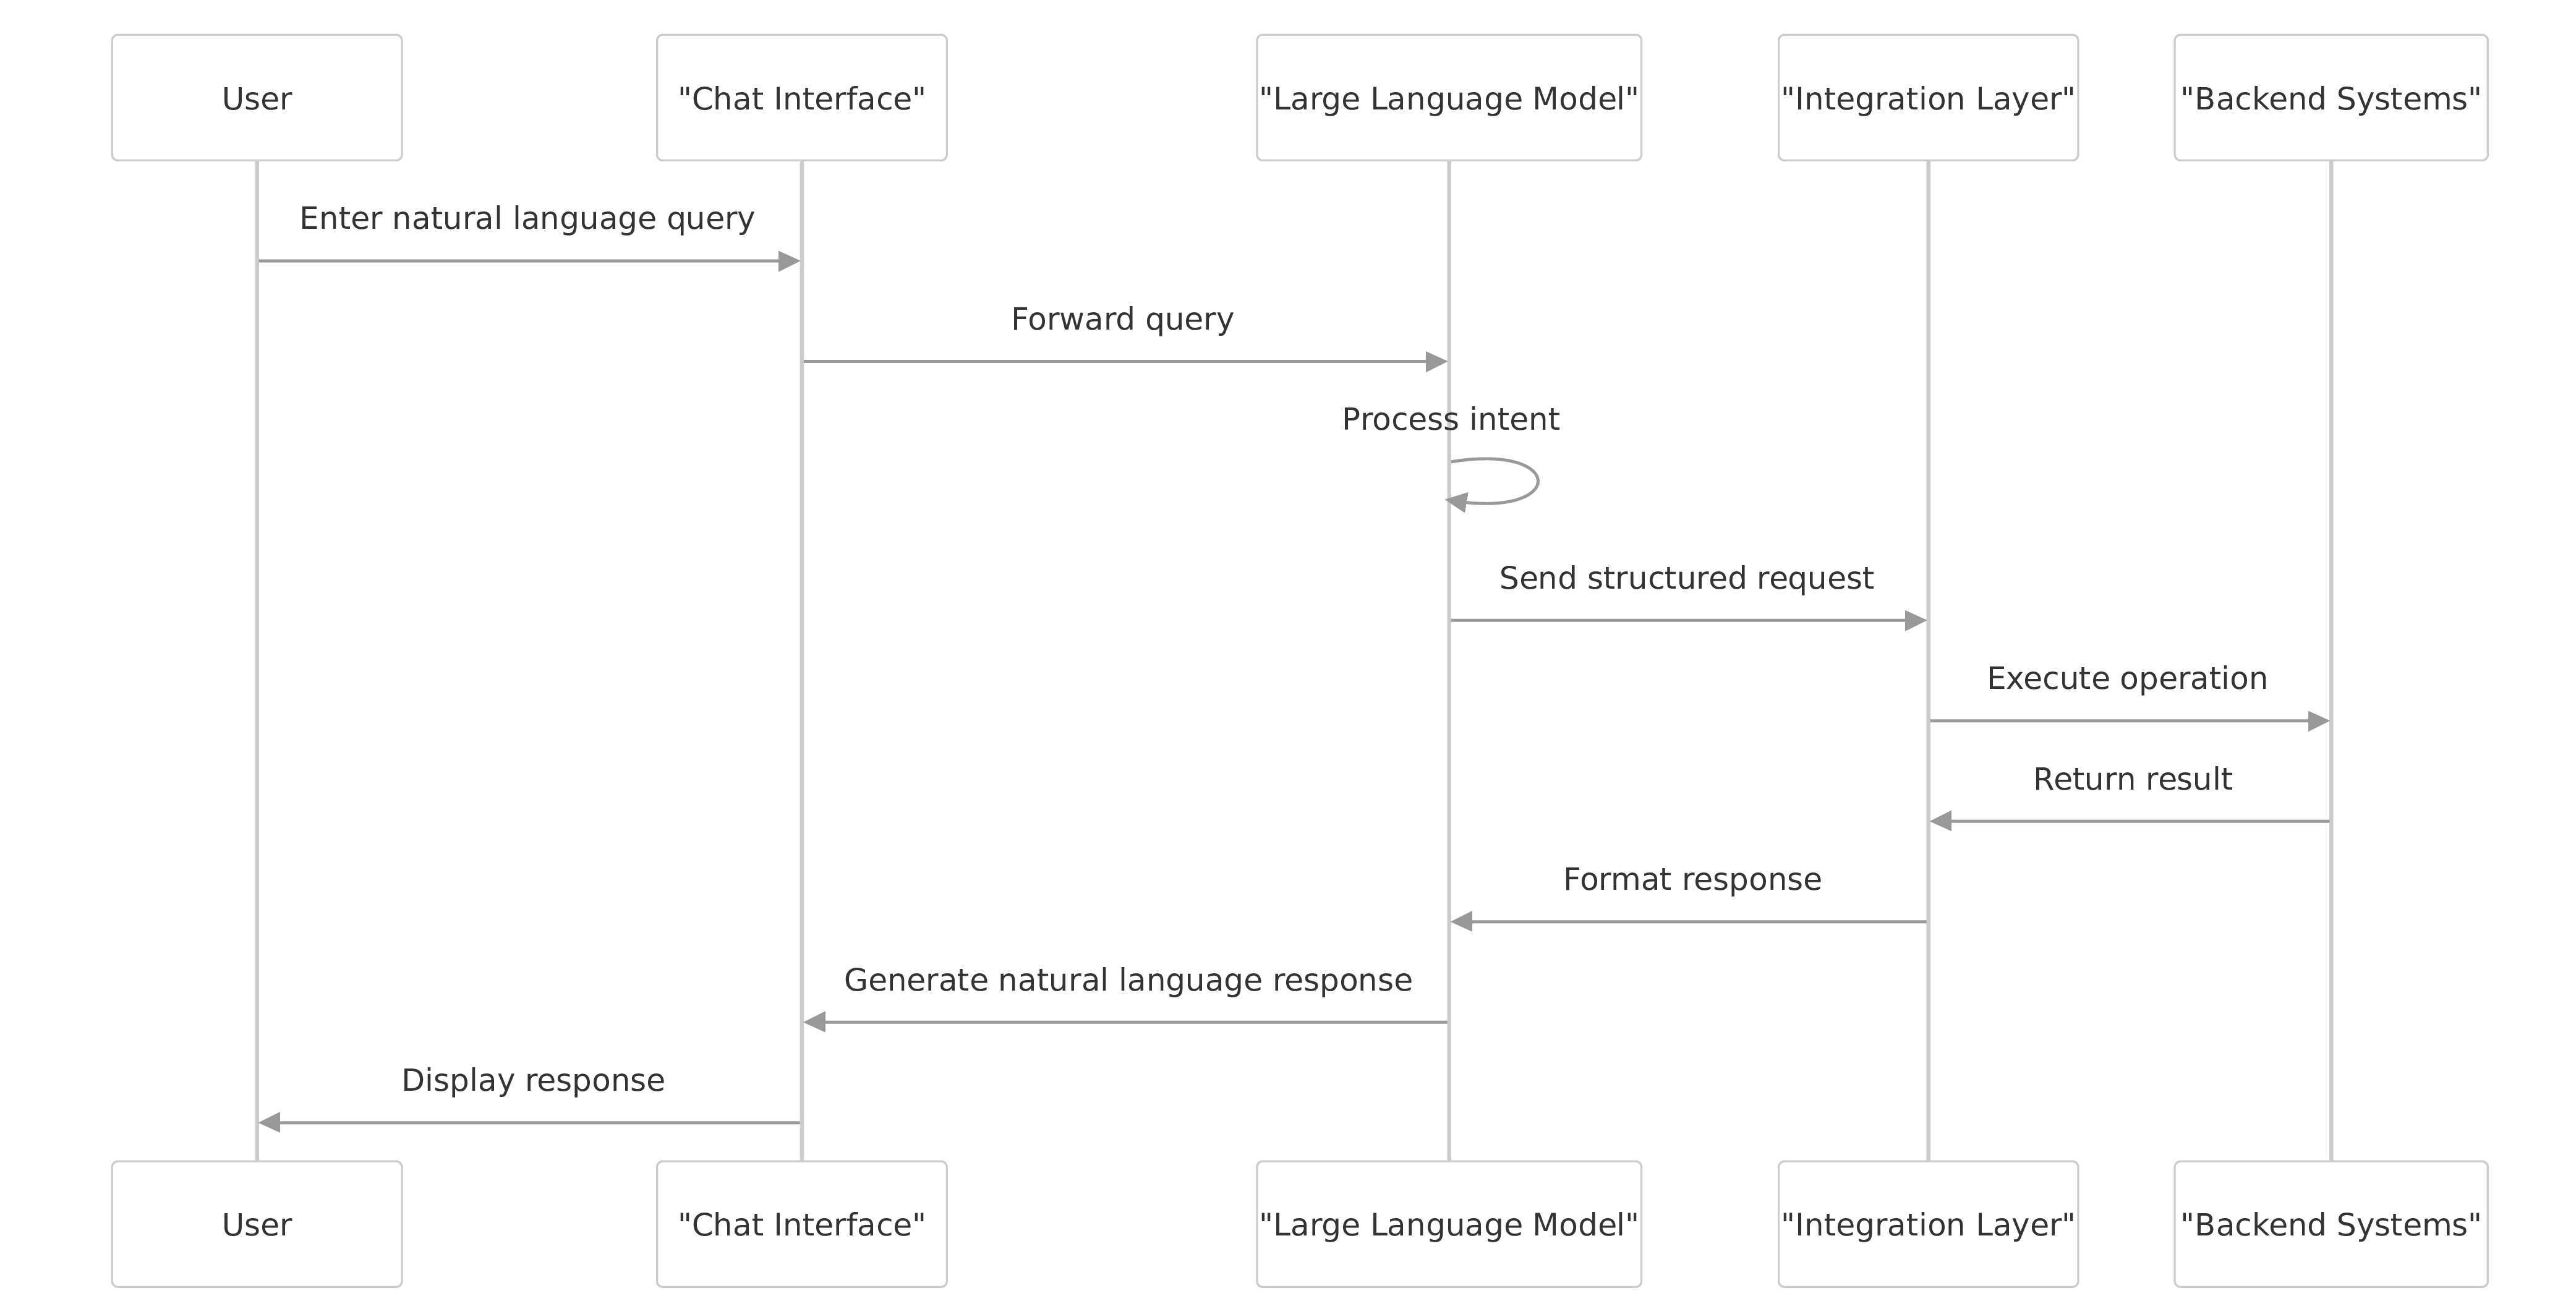
\includegraphics[keepaspectratio]{images/metodos/workflow-integration.jpg}}
\caption{Diagrama de Workflow do Agente}
\end{figure}

\subsubsection{2.2.3 Coleta de Métricas via Testes
E2E}\label{coleta-de-muxe9tricas-via-testes-e2e}

Testes End-to-End (E2E) são essenciais para avaliar não apenas o
desempenho e a segurança, mas também a experiência geral do usuário com
sistemas integrados a LLMs. Os testes são automatizados, executados
regularmente em ambiente controlado para assegurar resultados
consistentes e comparáveis.

Os testes envolvem: - Avaliação detalhada da performance, incluindo
tempos totais de resposta, tempo específico do processamento pelo modelo
de linguagem e latência da rede. - Análise da confiabilidade através da
taxa de sucesso das requisições e frequência de erros críticos e não
críticos. - Avaliação de segurança utilizando técnicas de \emph{Red
Team}, incluindo a tentativa sistemática de exploração de
vulnerabilidades com injeção de \emph{prompts} e validação dos controles
de acesso. - Mensuração da experiência do usuário, utilizando avaliações
qualitativas da clareza das respostas e pesquisas estruturadas de
satisfação com escalas Likert.

Os testes E2E são executados de forma automatizada em ambiente
controlado, simulando diferentes cenários de uso e condições de carga,
permitindo uma avaliação objetiva e reproduzível de cada abordagem de
integração.

Esta padronização da coleta de métricas via testes E2E garante que as
diferenças observadas entre as abordagens sejam resultado direto das
suas características de implementação, e não de variações na experiência
do usuário ou na forma de coleta de dados.

Em seguida, os testes são executados automaticamente, variando desde
consultas simples até cenários complexos e ataques adversários
simulados. As métricas obtidas são automaticamente registradas para
garantir uma coleta padronizada e confiável dos dados. Finalmente, uma
análise automatizada gera relatórios detalhados, permitindo uma
comparação objetiva e precisa entre as diferentes abordagens
implementadas.

\subsection{3. DESENVOLVIMENTO}\label{desenvolvimento}

\subsubsection{3.1 Integração via Plugin
ORM}\label{integrauxe7uxe3o-via-plugin-orm}

A primeira abordagem investigada consiste na implementação de um plugin
ORM que permite ao LLM interagir com o sistema através das camadas de
abstração do ORM. Esta seção detalha a arquitetura, implementação e
considerações práticas desta solução.

\paragraph{3.1.1 Arquitetura da
Solução}\label{arquitetura-da-soluuxe7uxe3o}

A arquitetura proposta para esta abordagem é composta por quatro
componentes principais: interface do usuário, serviço LLM, plugin ORM e
o banco de dados. A Figura X ilustra a arquitetura e o fluxo de
comunicação entre estes componentes.

\begin{figure}
\centering
\pandocbounded{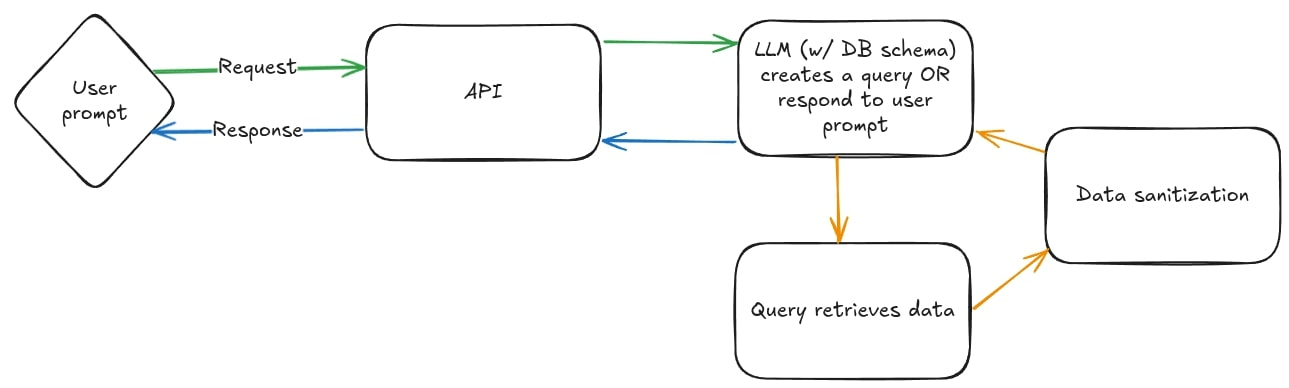
\includegraphics[keepaspectratio]{images/orm/orm-diagram-approach.jpg}}
\caption{ORM - Diagrama da Arquitetura}
\end{figure}

O fluxo de comunicação se inicia com uma solicitação do usuário em
linguagem natural, que é processada pelo LLM. O modelo, tendo
conhecimento prévio dos modelos e relacionamentos definidos no ORM, gera
instruções de consulta utilizando a API do ORM. Estas instruções são
executadas através do plugin, que utiliza o ORM para realizar as
operações no banco de dados de forma segura e otimizada.

Em casos mais complexos, o sistema pode realizar múltiplas operações
encadeadas, aproveitando os relacionamentos e métodos definidos nos
modelos do ORM para obter dados relacionados e realizar análises mais
complexas.

\paragraph{3.1.2 Componentes de
Segurança}\label{componentes-de-seguranuxe7a}

A implementação inclui camadas de segurança essenciais:

\begin{itemize}
\tightlist
\item
  Validação automática de tipos pelo ORM
\item
  Prevenção de \emph{SQL injection}
\item
  Controle de acesso em nível de modelo
\item
  Sanitização de dados de entrada
\item
  Validação de permissões de usuário
\end{itemize}

\paragraph{3.1.3 Estrutura de Metadados}\label{estrutura-de-metadados}

A configuração do sistema é gerenciada através dos modelos do ORM:

\begin{itemize}
\tightlist
\item
  Definições de modelos e relacionamentos
\item
  Validações e restrições de campo
\item
  Hooks e middlewares
\item
  Configurações de cache
\end{itemize}

\paragraph{3.1.4 Implementação da Prova de
Conceito}\label{implementauxe7uxe3o-da-prova-de-conceito}

A implementação utiliza uma stack tecnológica moderna baseada em
Node.js, escolhida por sua eficiência e amplo suporte a ferramentas de
desenvolvimento. Os principais componentes tecnológicos incluem:

\begin{itemize}
\tightlist
\item
  Backend: Node.js
\item
  LLM: GPT-3 via API OpenAI
\item
  ORM: Sequelize
\item
  Banco de Dados: PostgreSQL
\end{itemize}

\paragraph{3.1.5 Desenvolvimento do
Plugin}\label{desenvolvimento-do-plugin}

O plugin ORM implementa:

\begin{itemize}
\tightlist
\item
  Interface de comunicação com o LLM
\item
  Interpretação de intenções para queries
\item
  Gerenciamento de transações
\item
  Sistema de cache
\item
  Logging e monitoramento
\end{itemize}

\paragraph{3.1.6 Detalhes Técnicos}\label{detalhes-tuxe9cnicos}

A implementação técnica foca em três aspectos principais:

\paragraph{3.1.7 Integração com LLM}\label{integrauxe7uxe3o-com-llm}

O sistema utiliza técnicas avançadas de \emph{prompt engineering} para:

\begin{itemize}
\tightlist
\item
  Interpretação de modelos do ORM
\item
  Geração de queries complexas
\item
  Otimização de consultas
\item
  Gerenciamento de relacionamentos
\end{itemize}

\paragraph{3.1.8 Tratamento de Erros}\label{tratamento-de-erros}

O sistema implementa estratégias robustas para:

\begin{itemize}
\tightlist
\item
  Validação de tipos
\item
  Erros de constraint
\item
  Timeout de transações
\item
  Conflitos de concorrência
\end{itemize}

\paragraph{3.1.9 Avaliação e
Métricas}\label{avaliauxe7uxe3o-e-muxe9tricas}

Esta abordagem foi avaliada considerando os seguintes aspectos:

\begin{itemize}
\tightlist
\item
  Performance
\item
  Segurança
\item
  Custos Operacionais
\end{itemize}

\paragraph{3.1.10 Considerações
Práticas}\label{considerauxe7uxf5es-pruxe1ticas}

A implementação revelou diversos aspectos práticos importantes:

\begin{itemize}
\tightlist
\item
  Desafios
\item
  Infraestrutura
\item
  Manutenção
\end{itemize}

\subsubsection{3.2 Integração
OpenAPI-MCP}\label{integrauxe7uxe3o-openapi-mcp}

A terceira abordagem implementa uma solução unificada que combina a
especificação OpenAPI com o \emph{Model Context Protocol (MCP)}. Esta
seção detalha a arquitetura, implementação e considerações práticas
desta solução integrada.

\paragraph{3.2.1 Arquitetura da
Solução}\label{arquitetura-da-soluuxe7uxe3o-1}

A arquitetura proposta para esta abordagem implementa um servidor MCP
que é gerado a partir de uma definição OpenAPI e que pode ser integrado
a qualquer sistema que suporte o protocolo MCP. Dessa forma, a
integração é feita através de uma definição OpenAPI, que é a forma
padrão de se integrar sistemas através de APIs.

\begin{figure}
\centering
\pandocbounded{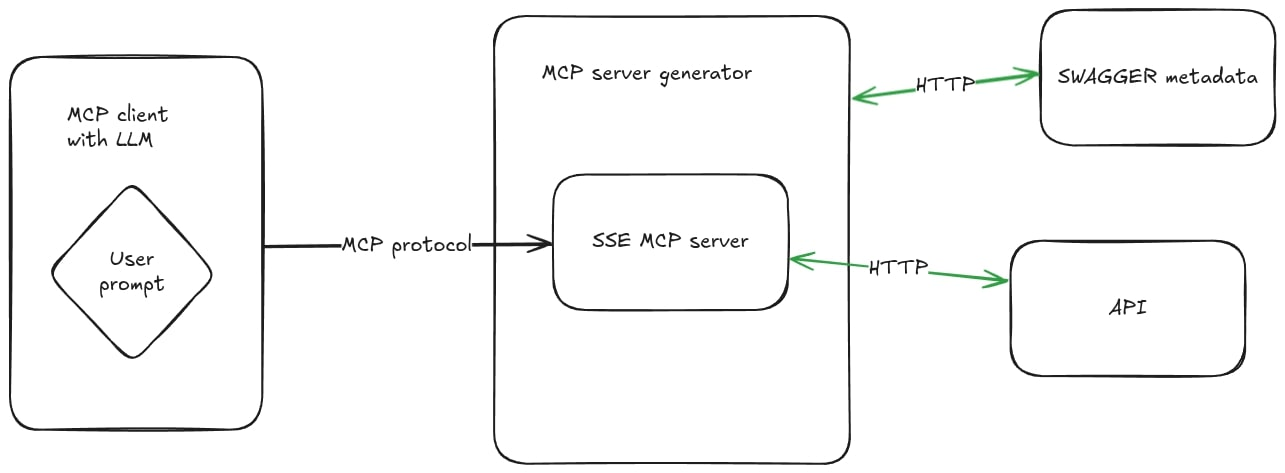
\includegraphics[keepaspectratio]{images/openapi-mcp/openapi-mcp-diagram-approach.jpg}}
\caption{OpenAPI-MCP - Diagrama da Arquitetura}
\end{figure}

A arquitetura desta abordagem é composta por três camadas principais:

\begin{enumerate}
\def\labelenumi{\arabic{enumi}.}
\item
  \textbf{Camada de Definição API}

  \begin{itemize}
  \tightlist
  \item
    Especificações OpenAPI dos sistemas alvo
  \item
    Definições de endpoints e operações
  \item
    Esquemas de dados e validação
  \item
    Configurações de segurança e autenticação
  \end{itemize}
\item
  \textbf{Camada de Geração MCP}

  \begin{itemize}
  \tightlist
  \item
    Gerador automático de servidores MCP
  \item
    Mapeamento OpenAPI para MCP
  \item
    Geradores de código
  \end{itemize}
\item
  \textbf{Camada de Runtime Cliente MCP}

  \begin{itemize}
  \tightlist
  \item
    Servidor MCP gerado
  \item
    Cliente MCP (LLM)
  \item
    Proxy de requisições REST
  \item
    Sistema de cache e otimização
  \end{itemize}
\end{enumerate}

\paragraph{3.2.2 Fluxo de Operação}\label{fluxo-de-operauxe7uxe3o}

O sistema opera através do seguinte fluxo:

\begin{enumerate}
\def\labelenumi{\arabic{enumi}.}
\tightlist
\item
  Definição das APIs via OpenAPI
\item
  Geração automática do servidor MCP
\item
  Processamento de \emph{prompts} do usuário pelo LLM
\item
  Tradução de intenções em chamadas MCP using SSE
\item
  Processamento das respostas e apresentação ao usuário
\end{enumerate}

\paragraph{3.2.3 Componentes de
Segurança}\label{componentes-de-seguranuxe7a-1}

A implementação mantém as características de segurança de ambos os
protocolos:

\begin{itemize}
\tightlist
\item
  Validação de schemas OpenAPI
\item
  Autenticação e gestão de permissões para uso do swagger
\end{itemize}

\paragraph{3.2.4 Implementação da Prova de
Conceito}\label{implementauxe7uxe3o-da-prova-de-conceito-1}

A implementação utiliza as seguintes tecnologias:

\begin{itemize}
\tightlist
\item
  Node.js para o servidor de geração
\item
  OpenAPI Tools para parsing de especificações
\item
  MCP SDK para geração de servidores
\end{itemize}

\paragraph{3.2.5 Desenvolvimento do
Gerador}\label{desenvolvimento-do-gerador}

O gerador de servidores MCP implementa:

\begin{itemize}
\tightlist
\item
  Parser de especificações OpenAPI
\item
  Mapeamento de tipos OpenAPI para MCP
\item
  Geração de código Typescript
\item
  Templates de servidores MCP
\item
  Sistema de plugins para extensibilidade
\end{itemize}

\paragraph{3.2.6 Detalhes Técnicos}\label{detalhes-tuxe9cnicos-1}

A implementação foca em três aspectos principais:

\begin{enumerate}
\def\labelenumi{\arabic{enumi}.}
\item
  \textbf{Geração de Código}

  \begin{itemize}
  \tightlist
  \item
    Análise estática de especificações
  \item
    Geração de tipos Typescript
  \item
    Criação de validadores
  \item
    Documentação automática
  \end{itemize}
\item
  \textbf{Runtime}

  \begin{itemize}
  \tightlist
  \item
    Tratamento de erros de chamadas MCP
  \end{itemize}
\item
  \textbf{Integração LLM}

  \begin{itemize}
  \tightlist
  \item
    \emph{Prompt engineering} para uso das ferramentas MCP
  \item
    Gerenciamento de contexto
  \item
    Otimização de chamadas
  \item
    Interpretação de respostas
  \end{itemize}
\end{enumerate}

\paragraph{3.2.7 Avaliação e
Métricas}\label{avaliauxe7uxe3o-e-muxe9tricas-1}

A avaliação considera aspectos específicos desta abordagem:

\begin{enumerate}
\def\labelenumi{\arabic{enumi}.}
\item
  \textbf{Performance}

  \begin{itemize}
  \tightlist
  \item
    Tempo de geração de servidores
  \item
    Latência de chamadas MCP
  \item
    Eficiência de cache
  \end{itemize}
\item
  \textbf{Confiabilidade}

  \begin{itemize}
  \tightlist
  \item
    Taxa de sucesso de geração
  \item
    Estabilidade do servidor
  \item
    Consistência das respostas
  \end{itemize}
\item
  \textbf{Manutenibilidade}

  \begin{itemize}
  \tightlist
  \item
    Facilidade de atualização
  \item
    Compatibilidade com versões
  \item
    Clareza do código gerado
  \item
    Documentação automática
  \end{itemize}
\end{enumerate}

\paragraph{3.2.8 Considerações
Práticas}\label{considerauxe7uxf5es-pruxe1ticas-1}

A implementação revelou aspectos importantes:

\begin{enumerate}
\def\labelenumi{\arabic{enumi}.}
\item
  \textbf{Desafios}

  \begin{itemize}
  \tightlist
  \item
    Complexidade de mapeamento de tipos
  \item
    Manutenção de estado entre chamadas
  \item
    Versionamento de \emph{APIs}
  \item
    Performance em grande escala
  \end{itemize}
\item
  \textbf{Infraestrutura}

  \begin{itemize}
  \tightlist
  \item
    Requisitos de deployment
  \item
    Escalabilidade horizontal
  \item
    Monitoramento distribuído
  \item
    Backup e recuperação
  \end{itemize}
\item
  \textbf{Manutenção}

  \begin{itemize}
  \tightlist
  \item
    Atualizações de especificações
  \item
    Regeneração de servidores
  \item
    Migração de dados
  \item
    Gestão de dependências
  \end{itemize}
\end{enumerate}

\subsubsection{3.3 Integração via conexão direta com o banco de
dados}\label{integrauxe7uxe3o-via-conexuxe3o-direta-com-o-banco-de-dados}

A terceira abordagem explora a integração direta entre o \emph{LLM} e o
banco de dados, minimizando camadas intermediárias de abstração. Esta
abordagem oferece máximo controle e performance, mas requer cuidados
especiais com segurança e validação. Esta seção detalha a arquitetura,
implementação e considerações práticas desta solução.

\paragraph{3.3.1 Arquitetura da
Solução}\label{arquitetura-da-soluuxe7uxe3o-2}

A arquitetura desta abordagem é intencionalmente minimalista, composta
por três componentes principais:

\begin{enumerate}
\def\labelenumi{\arabic{enumi}.}
\item
  \textbf{Camada de Interface}

  \begin{itemize}
  \tightlist
  \item
    Cadastro das conexões com o banco de dados (para que a aplicação
    possa obter os schemas e executar queries)
  \item
    Serviço \emph{LLM} (para gerar queries, interpretar os dados e gerar
    respostas)
  \end{itemize}
\item
  \textbf{Camada de Segurança}

  \begin{itemize}
  \tightlist
  \item
    Sistema de validação de queries (para sanitizar os dados e evitar
    \emph{SQL injection})
  \end{itemize}
\item
  \textbf{Camada de Dados}

  \begin{itemize}
  \tightlist
  \item
    Gerenciamento de conexões com o banco de dados (em caso de múltiplos
    databases, a aplicação deve integrar todos e possibilitar que o
    \emph{LLM} escolha qual usar)
  \item
    Cache de queries
  \end{itemize}
\end{enumerate}

\begin{figure}
\centering
\pandocbounded{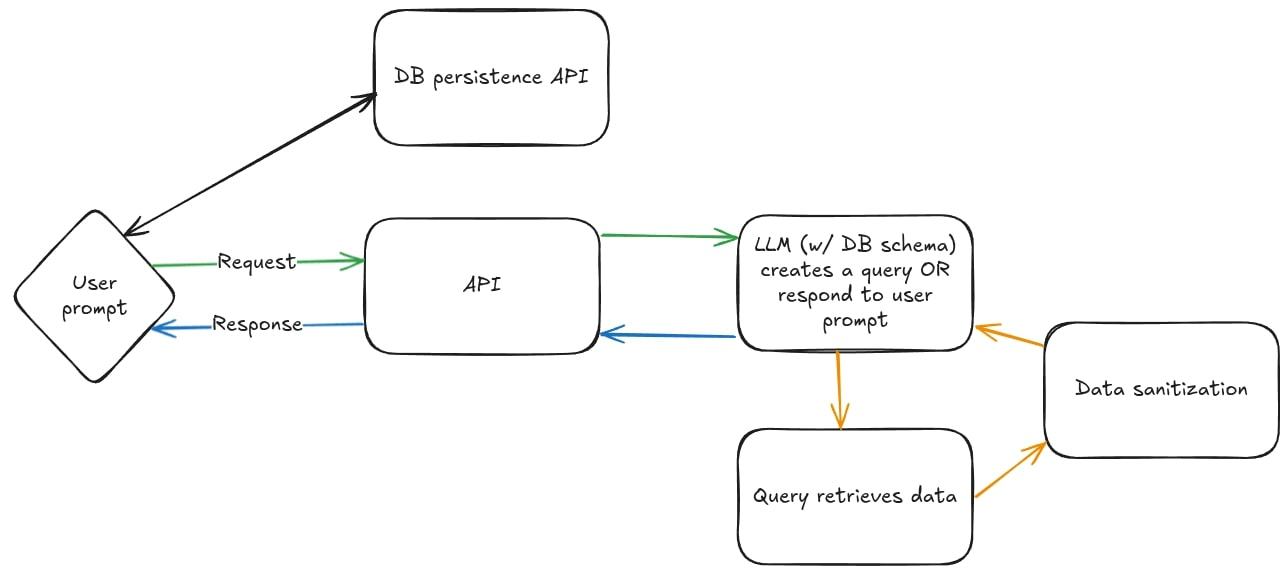
\includegraphics[keepaspectratio]{images/db/db-diagram-approach.jpg}}
\caption{DB - Diagrama da Arquitetura}
\end{figure}

\paragraph{3.3.2 Fluxo de Operação}\label{fluxo-de-operauxe7uxe3o-1}

O sistema opera através de um fluxo direto:

\begin{enumerate}
\def\labelenumi{\arabic{enumi}.}
\tightlist
\item
  Recebimento do prompt do usuário
\item
  Análise de intenção pelo \emph{LLM}
\item
  Geração de query \emph{SQL}
\item
  Validação e sanitização
\item
  Execução direta no banco
\item
  Processamento dos resultados
\item
  Formatação da resposta
\end{enumerate}

\paragraph{3.3.3 Componentes de
Segurança}\label{componentes-de-seguranuxe7a-2}

Dado o acesso direto ao banco, a segurança é crítica:

\begin{itemize}
\tightlist
\item
  Sistema robusto de sanitização \emph{SQL}
\item
  Análise estática de queries
\item
  Validação de tipos de dados
\item
  Limites de complexidade de query
\item
  Timeouts configuráveis
\end{itemize}

\paragraph{3.3.4 Implementação da Prova de
Conceito}\label{implementauxe7uxe3o-da-prova-de-conceito-2}

A implementação utiliza tecnologias focadas em performance:

\begin{itemize}
\tightlist
\item
  Backend: \emph{Node.js}
\item
  \emph{LLM}: GPT-3 via \emph{API} OpenAI
\item
  Banco de Dados: PostgreSQL
\item
  Driver: node-postgres
\item
  Sistema de Cache: Redis
\end{itemize}

\paragraph{3.3.5 Desenvolvimento do
Conector}\label{desenvolvimento-do-conector}

O conector de banco de dados implementa:

\begin{itemize}
\tightlist
\item
  Pool de conexões otimizado
\item
  Sistema de retry inteligente
\item
  Sanitização de queries
\item
  Cache adaptativo
\item
  Logging detalhado
\item
  Métricas em tempo real
\end{itemize}

\paragraph{3.3.6 Detalhes Técnicos}\label{detalhes-tuxe9cnicos-2}

A implementação foca em três aspectos críticos:

\begin{enumerate}
\def\labelenumi{\arabic{enumi}.}
\item
  \textbf{Geração de \emph{SQL}}

  \begin{itemize}
  \tightlist
  \item
    Templates de queries otimizadas
  \item
    Análise de plano de execução
  \item
    Otimização automática
  \item
    Validação sintática
  \end{itemize}
\item
  \textbf{Performance}

  \begin{itemize}
  \tightlist
  \item
    Connection pooling
  \item
    Query caching
  \item
    Bulk operations
  \item
    Índices automáticos
  \end{itemize}
\item
  \textbf{Segurança}

  \begin{itemize}
  \tightlist
  \item
    Análise de injeção \emph{SQL}
  \item
    Validação de schemas
  \item
    Rate limiting
  \item
    Auditoria de acessos
  \end{itemize}
\end{enumerate}

\paragraph{3.3.7 Avaliação e
Métricas}\label{avaliauxe7uxe3o-e-muxe9tricas-2}

A avaliação considera aspectos específicos:

\begin{enumerate}
\def\labelenumi{\arabic{enumi}.}
\item
  \textbf{Performance}

  \begin{itemize}
  \tightlist
  \item
    Latência de queries
  \item
    Throughput do sistema
  \item
    Uso de recursos
  \item
    Hit rate do cache
  \end{itemize}
\item
  \textbf{Segurança}

  \begin{itemize}
  \tightlist
  \item
    Taxa de detecção de injeção
  \item
    Cobertura de validação
  \item
    Eficácia do controle de acesso
  \item
    Precisão da auditoria
  \end{itemize}
\item
  \textbf{Confiabilidade}

  \begin{itemize}
  \tightlist
  \item
    Taxa de erros
  \item
    Tempo de recuperação
  \item
    Consistência dos dados
  \item
    Disponibilidade do sistema
  \end{itemize}
\end{enumerate}

\paragraph{3.3.8 Considerações
Práticas}\label{considerauxe7uxf5es-pruxe1ticas-2}

A implementação revelou aspectos importantes:

\begin{enumerate}
\def\labelenumi{\arabic{enumi}.}
\item
  \textbf{Desafios}

  \begin{itemize}
  \tightlist
  \item
    Complexidade de validação
  \item
    Gestão de conexões
  \item
    Otimização de queries
  \item
    Segurança robusta
  \end{itemize}
\item
  \textbf{Infraestrutura}

  \begin{itemize}
  \tightlist
  \item
    Alta disponibilidade
  \item
    Backup em tempo real
  \item
    Monitoramento intensivo
  \item
    Escalabilidade vertical
  \end{itemize}
\item
  \textbf{Manutenção}

  \begin{itemize}
  \tightlist
  \item
    Atualizações de schema
  \item
    Otimização contínua
  \item
    Análise de logs
  \item
    Gestão de índices
  \end{itemize}
\end{enumerate}

Esta abordagem, embora mais complexa em termos de segurança e
manutenção, oferece máxima flexibilidade e performance para casos de uso
específicos onde o controle direto sobre as operações de banco de dados
é necessário.

\section{4 RESULTADOS E DISCUSSÕES}\label{resultados-e-discussuxf5es}

Nos Resultados e Discussões, deve-se apresentar os resultados obtidos no
Procedimento Experimental e fazer uma discussão e análise sobre os
mesmos sempre que possível referenciando a literatura pesquisada.

\section{5 CONSIDERAÇÕES FINAIS}\label{considerauxe7uxf5es-finais}

Etapa esta que servirá para você evidenciar as conquistas alcançadas com
o estudo e indicar as limitações e as reconsiderações. Além disso, você
poderá apontar a relação entre fatos verificados e teoria e mostrar a
contribuição da pesquisa para o meio acadêmico, empresarial e/ou para o
desenvolvimento da ciência e tecnologia. Além disso, você poderá sugerir
temas complementares a sua pesquisa para estudos futuros. Responda aqui
a sua pergunta-problema de pesquisa.

\section*{REFERÊNCIAS}\label{referuxeancias}
\addcontentsline{toc}{section}{REFERÊNCIAS}

\phantomsection\label{refs}
\begin{CSLReferences}{0}{1}
\bibitem[\citeproctext]{ref-anthropic2024context}
ANTHROPIC. \textbf{Anthropic Now Offers 100K Context Windows for Claude
3 Models}. Disponível em:
\textless{}\url{https://www.anthropic.com/news/100k-context-windows}\textgreater.

\bibitem[\citeproctext]{ref-anthropic2024mcp}
ANTHROPIC. \textbf{Model Context Protocol (MCP): A Standard for AI
Context Integration}. Disponível em:
\textless{}\url{https://www.anthropic.com/news/model-context-protocol}\textgreater.
Acesso em: 12 abr. 2025a.

\bibitem[\citeproctext]{ref-Anthropic2024}
ANTHROPIC. \textbf{{Introducing the Model Context Protocol}}. Anthropic
News, nov. c2024. Disponível em:
\textless{}\url{https://www.anthropic.com/news/model-context-protocol}\textgreater{}

\bibitem[\citeproctext]{ref-RedHat2024LLMNode}
BLOG, R. H. D. \textbf{Building LLM Agents with Node.js}.
\url{https://developers.redhat.com/blog/2024/10/25/building-agents-large-language-modelsllms-and-nodejs},
2024.

\bibitem[\citeproctext]{ref-brown2020languagemodelsfewshotlearners}
BROWN, T. B. et al. \textbf{Language Models are Few-Shot Learners}.,
2020. Disponível em:
\textless{}\url{https://arxiv.org/abs/2005.14165}\textgreater{}

\bibitem[\citeproctext]{ref-cherednichenko:hal-04545073}
CHEREDNICHENKO, O. et al. \textbf{Selection of Large Language Model for
development of Interactive Chat Bot for SaaS Solutions}. Lviv, Ukraine:
2024. Disponível em:
\textless{}\url{https://hal.science/hal-04545073}\textgreater{}

\bibitem[\citeproctext]{ref-Deng2023AMA}
DENG, X. \href{https://api.semanticscholar.org/CorpusID:258259387}{A
More Accessible Web with Natural Language Interface}.
\textbf{Proceedings of the 20th International Web for All Conference},
2023.

\bibitem[\citeproctext]{ref-enterprisedb2023security}
ENTERPRISEDB. \textbf{EnterpriseDB Raises the Bar for Postgres Security
and Compliance}. Disponível em:
\textless{}\url{https://www.enterprisedb.com/news/enterprisedb-raises-bar-postgres-security-compliance}\textgreater.
Acesso em: 12 abr. 2025b.

\bibitem[\citeproctext]{ref-enterprisedb2023postgresql}
ENTERPRISEDB. \textbf{Postgres is the Most Admired Database in Stack
Overflow 2023 Survey}. Disponível em:
\textless{}\url{https://www.enterprisedb.com/blog/postgres-most-admired-database-in-stack-overflow-2023}\textgreater.
Acesso em: 12 abr. 2025a.

\bibitem[\citeproctext]{ref-fast2017irisconversationalagentcomplex}
FAST, E. et al. \textbf{Iris: A Conversational Agent for Complex
Tasks}., 2017. Disponível em:
\textless{}\url{https://arxiv.org/abs/1707.05015}\textgreater{}

\bibitem[\citeproctext]{ref-Guo2024Doppelganger}
GUO, S. et al. \textbf{Collaborating with my Doppelgänger: The Effects
of Self-similar Appearance and Voice of a Virtual Character during a
Jigsaw Puzzle Co-solving Task}. Proceedings of the ACM on Computer
Graphics and Interactive Techniques. \textbf{Anais}...2024. Disponível
em:
\textless{}\url{https://www.researchgate.net/publication/335223260_The_Effects_of_Continuous_Conversation_and_Task_Complexity_on_Usability_of_an_AI-Based_Conversational_Agent_in_Smart_Home_Environments}\textgreater{}

\bibitem[\citeproctext]{ref-inie2025summon}
INIE, N.; STRAY, J.; DERCZYNSKI, L.
\href{https://journals.plos.org/plosone/article?id=10.1371/journal.pone.0314658}{Summon
a demon and bind it: A grounded theory of LLM red teaming}. \textbf{PloS
one}, v. 20, n. 1, p. e0314658, 2025.

\bibitem[\citeproctext]{ref-john2025owasp}
JOHN, S. et al.
\textbf{\href{https://genai.owasp.org/llmrisk/llm01-prompt-injection}{OWASP
Top 10 for LLM Apps \& Gen AI Agentic Security Initiative}}. tese de
doutorado---{[}s.l.{]} OWASP, 2025.

\bibitem[\citeproctext]{ref-Kocaballi2019}
KOCABALLI, A. B. et al. \href{https://doi.org/10.2196/15360}{The
Personalization of Conversational Agents in Health Care: Systematic
Review}. \textbf{J Med Internet Res}, v. 21, n. 11, p. e15360, 7 nov.
2019.

\bibitem[\citeproctext]{ref-Lister2020AccessibleCU}
LISTER, K. et al.
\href{https://api.semanticscholar.org/CorpusID:218539971}{Accessible
conversational user interfaces: considerations for design}.
\textbf{Proceedings of the 17th International Web for All Conference},
2020.

\bibitem[\citeproctext]{ref-MCPDocs2024}
MODEL CONTEXT PROTOCOL CONTRIBUTORS. \textbf{{Model Context Protocol
Documentation - Introduction}}. Online Documentation, 2024. Disponível
em:
\textless{}\url{https://modelcontextprotocol.io/introduction}\textgreater{}

\bibitem[\citeproctext]{ref-mcp2025spec}
MODEL CONTEXT PROTOCOL TEAM. \textbf{Model Context Protocol
Specification}. {[}s.l.{]} Model Context Protocol, 26 mar. 2025.
Disponível em:
\textless{}\url{https://modelcontextprotocol.io/specification/2025-03-26/index}\textgreater.
Acesso em: 12 abr. 2025.

\bibitem[\citeproctext]{ref-openai2022instructgpt}
OPENAI. \textbf{Aligning Language Models to Follow Instructions}.
{[}s.l.{]} OpenAI, 27 jan. 2022. Disponível em:
\textless{}\url{https://openai.com/index/instruction-following/}\textgreater.
Acesso em: 12 abr. 2025.

\bibitem[\citeproctext]{ref-openai2023gpt4}
OPENAI. \textbf{GPT-4 Research}. {[}s.l.{]} OpenAI, a2023. Disponível
em:
\textless{}\url{https://openai.com/index/gpt-4-research/}\textgreater.

\bibitem[\citeproctext]{ref-openai2023functioncalling}
OPENAI. \textbf{Function Calling and Other API Updates}. Disponível em:
\textless{}\url{https://openai.com/index/function-calling-and-other-api-updates/}\textgreater.
Acesso em: 12 abr. 2025b.

\bibitem[\citeproctext]{ref-OpenAI2023}
OPENAI. \textbf{{ChatGPT plugins}}. OpenAI Product Blog, mar. c2023.
Disponível em:
\textless{}\url{https://openai.com/blog/chatgpt-plugins}\textgreater{}

\bibitem[\citeproctext]{ref-OpenAPIInitiative2023}
OPENAPI INITIATIVE. \textbf{{OpenAPI Specification - Getting Started}}.
OpenAPI Documentation (openapis.org), 2023. Disponível em:
\textless{}\url{https://learn.openapis.org/docs/getting-started}\textgreater{}

\bibitem[\citeproctext]{ref-oprea2023adversarial}
OPREA, A.; VASSILEV, A. \textbf{Adversarial machine learning: A taxonomy
and terminology of attacks and mitigations}. {[}s.l.{]} National
Institute of Standards; Technology, 2023. Disponível em:
\textless{}\url{https://csrc.nist.gov/pubs/ai/100/2/e2023/final}\textgreater.

\bibitem[\citeproctext]{ref-RAPP201849}
RAPP, A. et al.
\href{https://doi.org/10.1016/j.ijhcs.2018.07.005}{Designing technology
for spatial needs: Routines, control and social competences of people
with autism}. \textbf{International Journal of Human-Computer Studies},
v. 120, p. 49--65, 2018.

\bibitem[\citeproctext]{ref-eversql2023orms}
TEAM, E. \textbf{Best ORM for Node.js in 2023: A Comprehensive
Comparison}. Disponível em:
\textless{}\url{https://www.eversql.com/best-orm-for-node-js/}\textgreater.
Acesso em: 12 abr. 2025.

\bibitem[\citeproctext]{ref-sequelize2024}
TEAM, S. \textbf{Sequelize: A Modern TypeScript and Node.js ORM for
Postgres, MySQL, MariaDB, SQLite and SQL Server}., 2024. Disponível em:
\textless{}\url{https://github.com/sequelize/sequelize}\textgreater.
Acesso em: 12 abr. 2025

\bibitem[\citeproctext]{ref-Postman2023}
THE POSTMAN TEAM. \textbf{{What is OpenAPI?}} Postman Blog, ago. 2023.
Disponível em:
\textless{}\url{https://blog.postman.com/what-is-openapi/}\textgreater{}

\bibitem[\citeproctext]{ref-wei2023chainofthoughtpromptingelicitsreasoning}
WEI, J. et al. \textbf{Chain-of-Thought Prompting Elicits Reasoning in
Large Language Models}., 2023. Disponível em:
\textless{}\url{https://arxiv.org/abs/2201.11903}\textgreater{}

\bibitem[\citeproctext]{ref-wu2023defending}
WU, F. et al.
\href{https://www.researchsquare.com/article/rs-2873090/v1}{Defending
chatgpt against jailbreak attack via self-reminder}. 2023.

\bibitem[\citeproctext]{ref-yao2023treethoughtsdeliberateproblem}
YAO, S. et al. \textbf{Tree of Thoughts: Deliberate Problem Solving with
Large Language Models}., 2023. Disponível em:
\textless{}\url{https://arxiv.org/abs/2305.10601}\textgreater{}

\end{CSLReferences}

\end{document}
